% Created 2022-03-08 mar. 12:35
% Intended LaTeX compiler: pdflatex
\documentclass[11pt]{article}
\usepackage[utf8]{inputenc}
\usepackage[T1]{fontenc}
\usepackage{graphicx}
\usepackage{grffile}
\usepackage{longtable}
\usepackage{wrapfig}
\usepackage{rotating}
\usepackage[normalem]{ulem}
\usepackage{amsmath}
\usepackage{textcomp}
\usepackage{amssymb}
\usepackage{capt-of}
\usepackage{hyperref}
\usepackage[usenames,dvipsnames]{color}
\usepackage{listings}
\usepackage[a4paper,left=2cm,right=2cm,top=2cm,bottom=2cm]{geometry}
\author{Cliquot Théo \& Marie Bornet}
\date{\today}
\title{Compte Rendu SDD calendrier}
\hypersetup{
 pdfauthor={Cliquot Théo \& Marie Bornet},
 pdftitle={Compte Rendu SDD calendrier},
 pdfkeywords={},
 pdfsubject={},
 pdfcreator={Emacs 26.3 (Org mode 9.4.6)}, 
 pdflang={English}}
\begin{document}

\maketitle
\tableofcontents


\section{Présentation générale}
\label{sec:org1a4716e}

\subsection{Objet du TP}
\label{sec:orgdc848c9}
\begin{quote}
On gère un échéancier (ou un agenda) grâce à une liste chaînée à deux niveaux.
\end{quote}

Le but de ce TP est de concevoir un emploi du temps consistant en des semaines
et chaque semaine pouvant contenir plusieurs actions. On doit pouvoir réaliser
des actions basiques avec ce calendrier, notamment afficher, ajouter ou
supprimer des actions, charger ou sauvegarder un calendrier depuis un fichier
\ldots{}
Pour cela, on va se servir d'une structure de données déjà vue en cours : la
liste chaînée.


\subsection{Les structures de données}
\label{sec:orgcf1e9f9}

\subsubsection{Action}
\label{sec:org2b26dcb}

L'action est caractérisée par un jour de la semaine et une heure, on donne à
chaque action un nom permettant de l'identifier facilement en moins de 10
caractères.


Dans le cadre d'un calendrier, ne pouvoir contrôler qu'une seule action ne nous
intéresse pas. C'est pour cela qu'on va préférer gérer une liste d'actions. Il va donc nous falloir, en plus des informations propres à chaque action, un nouveau
champ que l'on va nommer "suivant", qui va nous indiquer s'il y a une autre
action de prévue après celle en cours.

\lstset{morekeywords={main, printf, include, week_t, action_t, Pile,
File, Arbre},backgroundcolor=\color[rgb]{0.96,0.95,0.98},keywordstyle=\color[rgb]{0.627,0.126,0.941},commentstyle=\color[rgb]{0.233,0.8,0.233},stringstyle=\color[rgb]{1,0,0},keepspaces=true,deletekeywords={ps,scan},basicstyle=\ttfamily,numbers=left,breaklines=true,frame=lines,tabsize=4,language=C,label= ,caption= ,captionpos=b}
\begin{lstlisting}
typedef struct action {
  char day;            // Jour de la semaine (de 1 a 7)
  char hour[3];        // Heure (de 00 a 24)
  char name[10];       // nom de l'action
  struct action *suiv; // action suivante
} action_t;
\end{lstlisting}

En ce qui concerne la liste d'actions, on va utiliser une tête réelle qui pointera
vers la tête de notre liste. Ainsi une liste d'actions n'est pas à proprement
parler une structure, cependant on va utiliser un define pour la créer.

\lstset{morekeywords={main, printf, include, week_t, action_t, Pile,
File, Arbre},backgroundcolor=\color[rgb]{0.96,0.95,0.98},keywordstyle=\color[rgb]{0.627,0.126,0.941},commentstyle=\color[rgb]{0.233,0.8,0.233},stringstyle=\color[rgb]{1,0,0},keepspaces=true,deletekeywords={ps,scan},basicstyle=\ttfamily,numbers=left,breaklines=true,frame=lines,tabsize=4,language=C,label= ,caption= ,captionpos=b}
\begin{lstlisting}
#define listAction_t action_t *
\end{lstlisting}

Une seule action peut avoir le même jour et la même heure dans la même liste (on peut avoir 2 cours sur le même crenau et le même jour par exemple)

\begin{figure}[htbp]
\centering
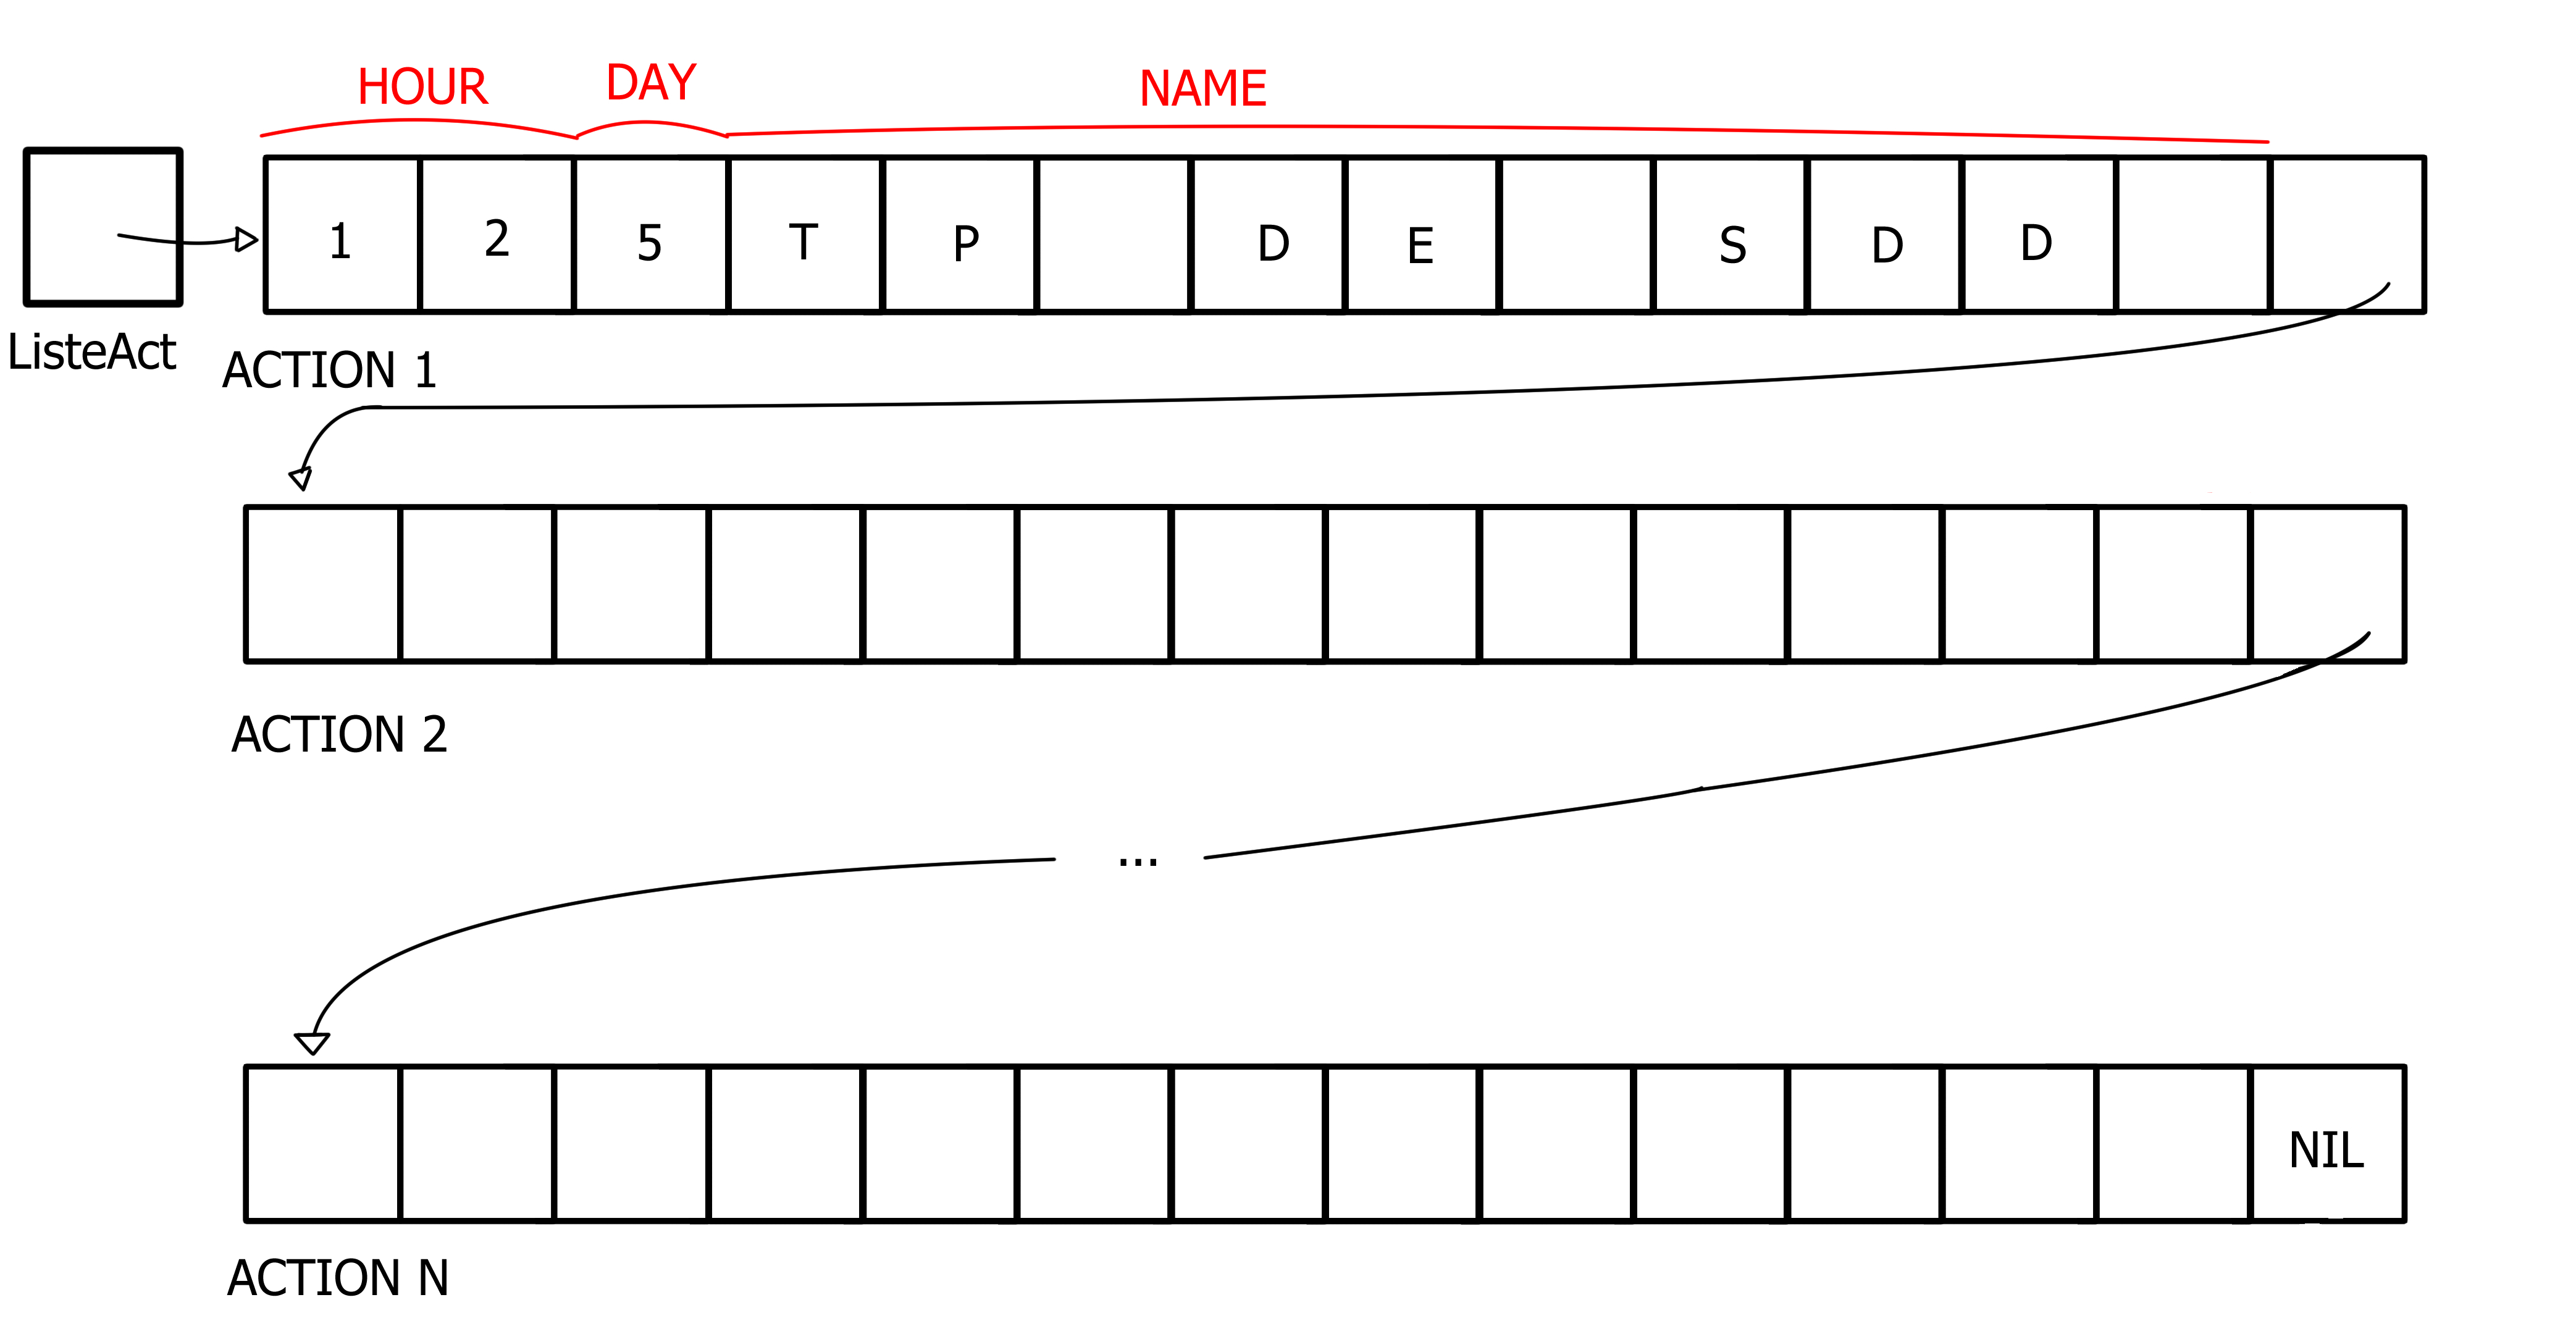
\includegraphics[width=.9\linewidth]{./act.jpg}
\caption{\label{fig:org76f1275}Schéma d'une action}
\end{figure}

\subsubsection{Semaine}
\label{sec:org40e960d}

La semaine se rapproche très fortement dans sa construction avec la structure action. En effet, on va gérer une semaine de la même façon que l'on gère une action, c'est-à-dire qu'une semaine sera une cellule, ce qui nous permettra de créer une liste de semaines. Une semaine sera aussi unique dans
une liste en fonction de son année et de son numéro.

Une semaine est constituée, comme dit précédemment, d'une année, d'un numéro de semaine mais aussi d'un pointeur vers la semaine qui suit celle en cours et d'une liste d'actions, représentant les actions à faire pour cette semaine.

\lstset{morekeywords={main, printf, include, week_t, action_t, Pile,
File, Arbre},backgroundcolor=\color[rgb]{0.96,0.95,0.98},keywordstyle=\color[rgb]{0.627,0.126,0.941},commentstyle=\color[rgb]{0.233,0.8,0.233},stringstyle=\color[rgb]{1,0,0},keepspaces=true,deletekeywords={ps,scan},basicstyle=\ttfamily,numbers=left,breaklines=true,frame=lines,tabsize=4,language=C,label= ,caption= ,captionpos=b}
\begin{lstlisting}
  typedef struct week {
  char year[5];         // Annee de la semaine
  char numWeek[3];      // Jour de la semaine (01 a 53)
  struct week *suiv;    // Semaine suivante
  listAction_t listAct; // Actions de la semaine
} week_t;

#define listWeek_t week_t *
\end{lstlisting}

Un choix a été fait dans action et semaine de séparer le jour de l'heure (pour action) et l'année du numéro de semaine (pour la semaine) pour des raisons de modularité et d'affichage. L'inconvénient étant que cette séparation nous force, dans certaines parties de notre code, à dupliquer les comparaisons, ce qui a pour effet de l'alourdir. Elle nous semblait cependant avantageuse du point de vue de la compréhension globale du code, en plus d'être beaucoup plus simple à modifier si on voulait changer la façon dans nos attributs sont stockés.

En ce qui concerne la façon dont sont stockés les différents attributs, nous avons privilégié les caractères (char) aux entiers (int) pour des raisons d'occupations de la mémoire. En effet, 2 ou 3 caractères prennent moins de place qu'un entier, et ceux-ci suffisent amplement.


\subsection{Les fichiers de données}
\label{sec:org2746676}

Les seuls fichiers de données nécessaires dans notre cas (entrée comme
sortie) sont ceux décrit dans l'énoncé

\begin{quote}
fichier texte où chaque ligne donne, sans séparateur :

année, semaine, jour, heure (sans espace), libellé de l’action sur 10 caractères
(complété avec des espaces si besoin)

Exemple de ligne : 202215108TPs de SDD
\end{quote}

En voici un exemple que l'on a utilisé pour tester notre programme :

\begin{verbatim}
202215108TP DE SDD
202315108prog_fonc
201015108COUCOU
202215108TP DE SDD
200007504TP CSN
200007510TP CSN2
202315310prog_fonc2
\end{verbatim}


\subsection{Organisation du code source}
\label{sec:org383da39}

Le code source est divisé en 4 fichiers (+ quelques fichiers headers pour connecter le tout). Les commentaires expliquant les fonctions se trouvent dans les headers pour des raisons de lisibilité.

\begin{figure}[htbp]
\centering
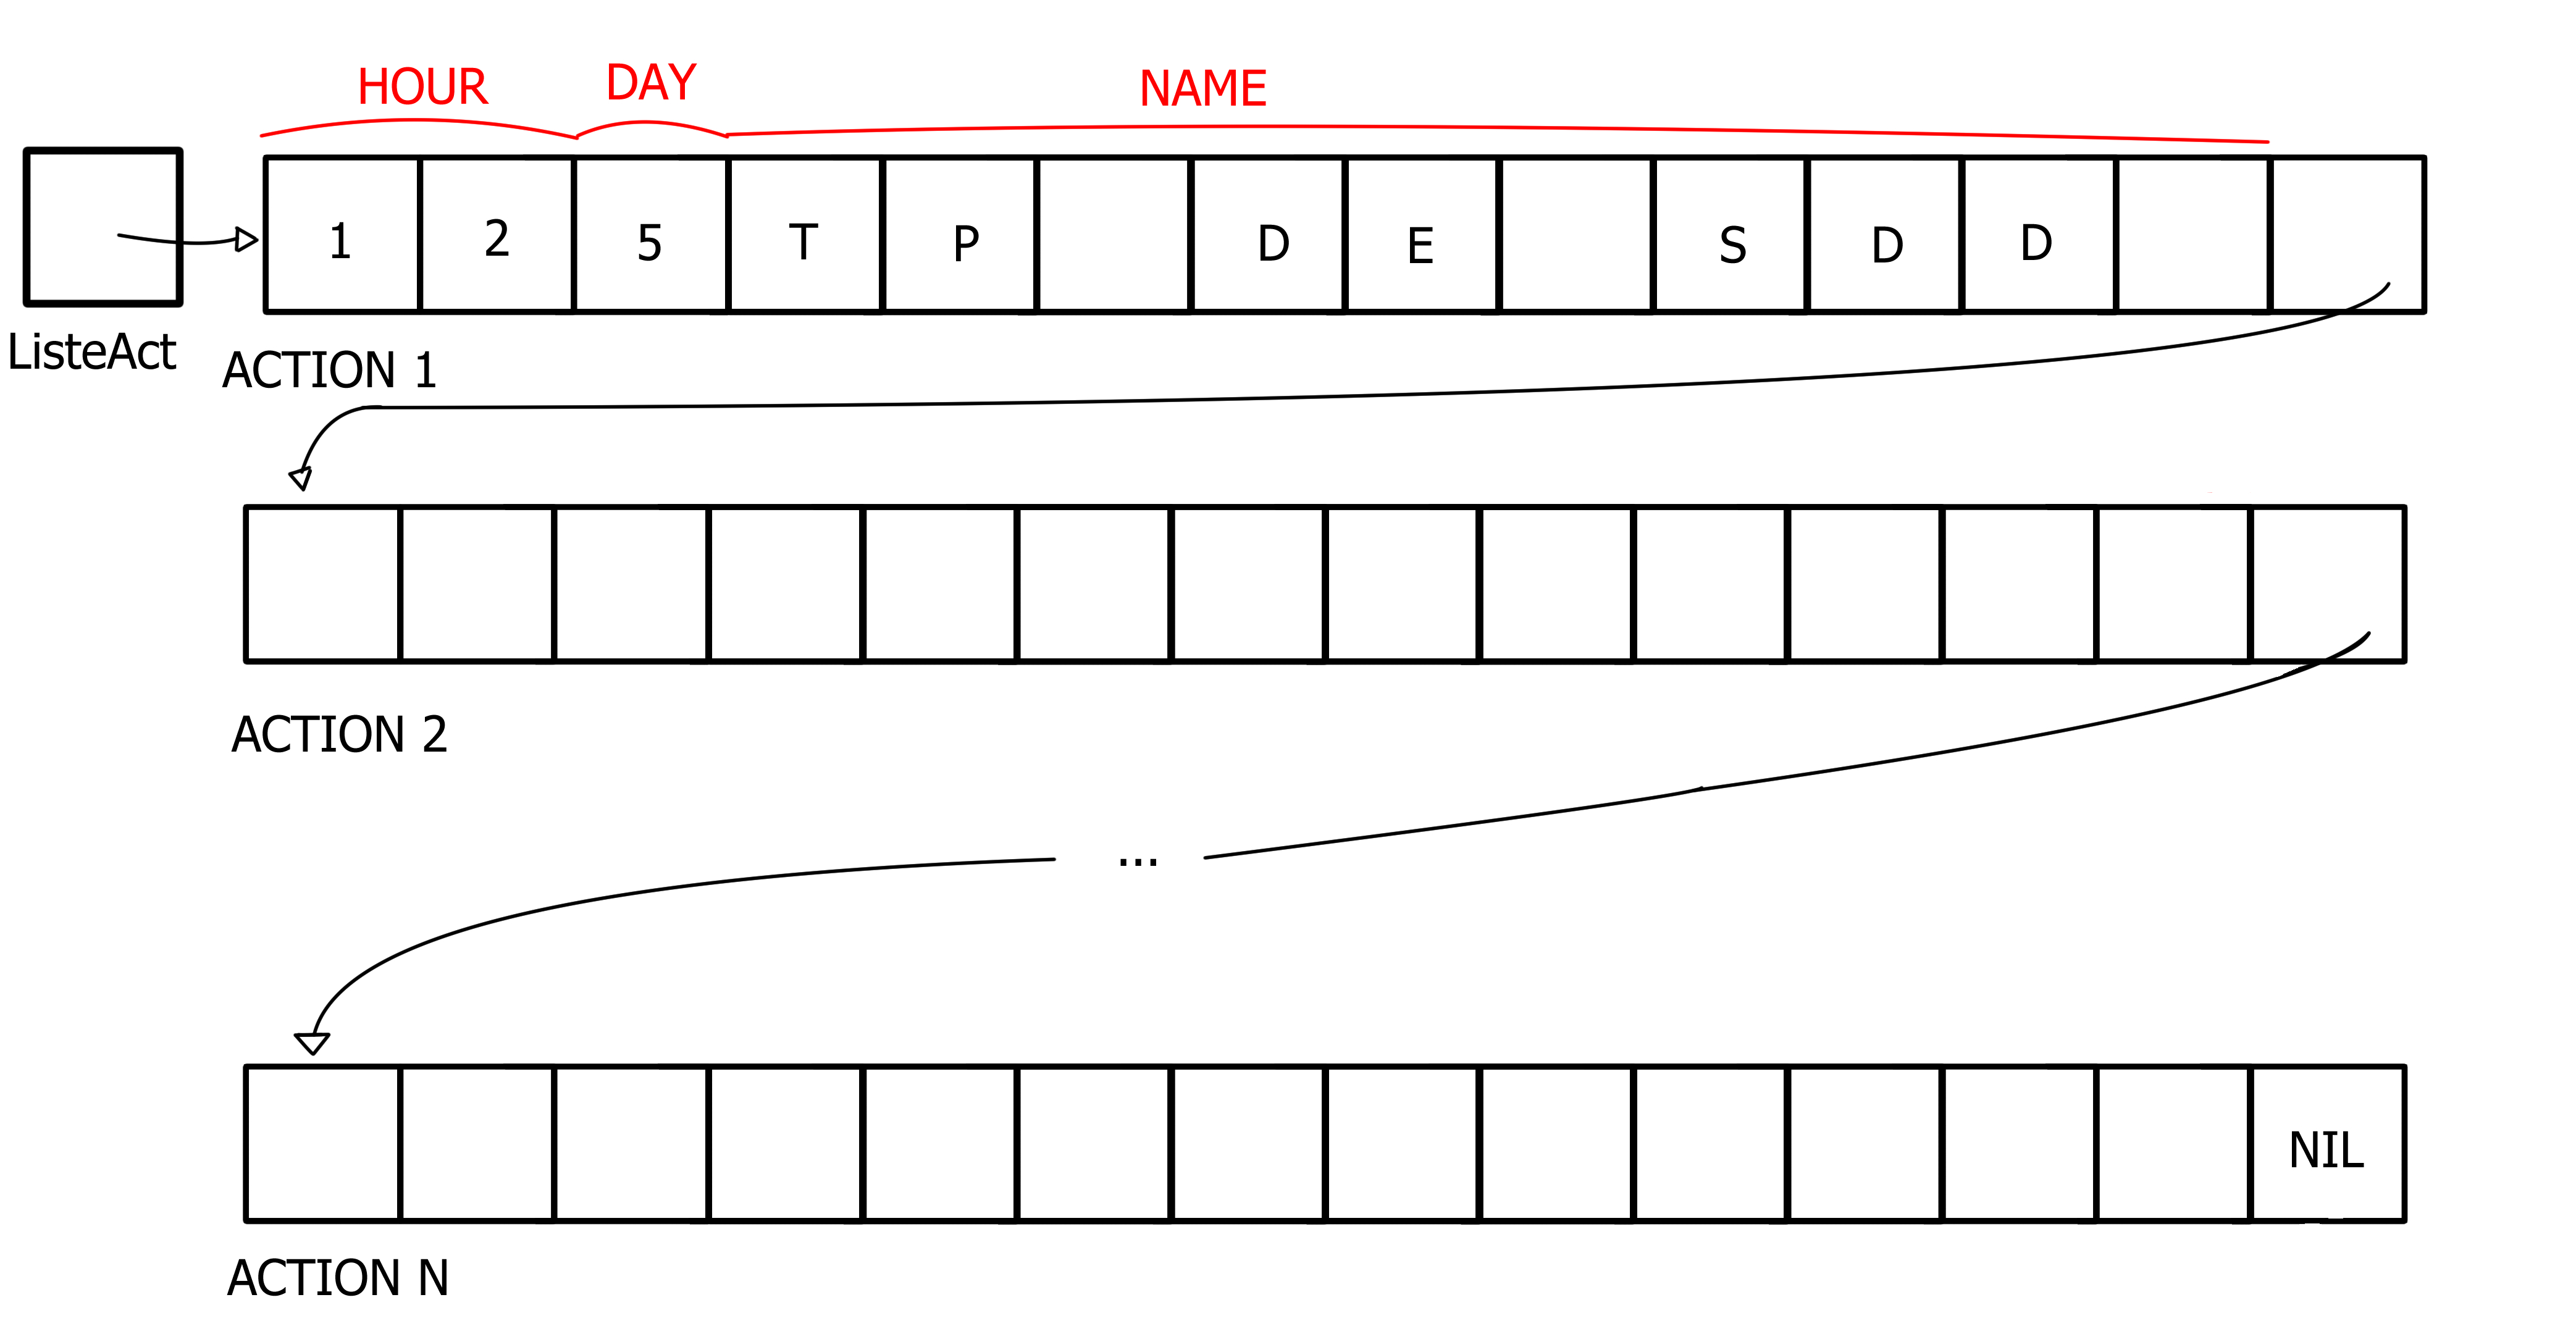
\includegraphics[width=.9\linewidth]{./sem.jpg}
\caption{\label{fig:org4cee2cc}Schéma d'une semaine}
\end{figure}

\subsubsection{Action.c}
\label{sec:orge407d73}

Ce fichier contient la déclaration de la structure action (définie plus tôt)
ainsi que toutes les fonctions se rapportant à celle-ci, On a notamment les
fonctions permettant d'allouer et de libérer une action, de la chercher, insérer
ou supprimer d'une liste, de la comparer avec une autre et enfin d'afficher
une liste d'actions de façon propre.


\subsubsection{semaine.c}
\label{sec:orgbc14bef}

Ce fichier contient la déclaration de la structure semaine (définie plus tôt) ainsi que toutes les fonctions se rapportant à celle-ci. On a exactement les mêmes fonctions que celles vues précédemment pour les actions et pour les semaines, ainsi que quelques fonctions supplémentaires provenant du fait que les actions font partie des semaines. On a donc, en plus des fonctions pour chercher, supprimer ou insérer des actions dans une liste de semaines.


\subsubsection{main.c}
\label{sec:org59b5416}

Ce fichier contient Le menu afin de gérer de façon claire et simplifiée la
gestion de notre calendrier. C'est notamment dans ce fichier que tout ce qui
concerne la lecture ou écriture du calendrier depuis un fichier et faite.
Pour le compiler il suffit d'utiliser la commande make afin d'appeler le
makefile (cf : makefile).

\subsubsection{test.c}
\label{sec:org4c95a96}

Ce fichier contient tous les jeux de tests afin de vérifier que nos différentes fonctions produisent bien le résultat escompté. Pour le compiler il suffit d'appeler le makefile avec comme argument test (cf : makefile)


\section{Fonctions}
\label{sec:org2a362a5}

Afin d'avoir une explication générale des fonctions, de leurs paramètres et de
leur sortie, un bloc de commentaire est déjà présent dans chaque headers. Cette
section s'intéresse plus au corps des fonctions et explique l'algorithme ainsi
que les différentes notations.

\subsection{Fonctions actions}
\label{sec:org787e83f}

\subsubsection{Sous procédures}
\label{sec:org0d0ab39}

\begin{enumerate}
\item checkDay
\label{sec:orgb340921}

CheckDay est une fonction présente pour simplifier la vérification et
rendre plus lisible les conditions dans les autres fonctions. Elle vérifie
seulement si le jour donné en argument \textbf{day} est cohérent.

\lstset{morekeywords={main, printf, include, week_t, action_t, Pile,
File, Arbre},backgroundcolor=\color[rgb]{0.96,0.95,0.98},keywordstyle=\color[rgb]{0.627,0.126,0.941},commentstyle=\color[rgb]{0.233,0.8,0.233},stringstyle=\color[rgb]{1,0,0},keepspaces=true,deletekeywords={ps,scan},basicstyle=\ttfamily,numbers=left,breaklines=true,frame=lines,tabsize=4,language=C,label= ,caption= ,captionpos=b}
\begin{lstlisting}
int checkDay(char day) { return (day > '0' && day < '7'); }
\end{lstlisting}


\item checkHour
\label{sec:org73b5817}

CheckHour est exactement la même fonction que checkDay mais pour les heures
\lstset{morekeywords={main, printf, include, week_t, action_t, Pile,
File, Arbre},backgroundcolor=\color[rgb]{0.96,0.95,0.98},keywordstyle=\color[rgb]{0.627,0.126,0.941},commentstyle=\color[rgb]{0.233,0.8,0.233},stringstyle=\color[rgb]{1,0,0},keepspaces=true,deletekeywords={ps,scan},basicstyle=\ttfamily,numbers=left,breaklines=true,frame=lines,tabsize=4,language=C,label= ,caption= ,captionpos=b}
\begin{lstlisting}
  int checkHour(char hour[2]) {
  return strcmp(hour, "00") >= 0 && strcmp(hour, "24") <= 0;
}
\end{lstlisting}


\item compareAction
\label{sec:org8fcdeab}
CompareAction va comme indiquer dans le bloc de commentaire renvoyer 1 si
l'action donné en argument \textbf{act} viens avant où est égal chronologiquement avec la date
de référence \textbf{day} et \textbf{hour}.
\lstset{morekeywords={main, printf, include, week_t, action_t, Pile,
File, Arbre},backgroundcolor=\color[rgb]{0.96,0.95,0.98},keywordstyle=\color[rgb]{0.627,0.126,0.941},commentstyle=\color[rgb]{0.233,0.8,0.233},stringstyle=\color[rgb]{1,0,0},keepspaces=true,deletekeywords={ps,scan},basicstyle=\ttfamily,numbers=left,breaklines=true,frame=lines,tabsize=4,language=C,label= ,caption= ,captionpos=b}
\begin{lstlisting}
  int compareAction(action_t *act, char day, char hour[2]) {
  return act->day < day || (act->day == day && strcmp(act->hour, hour) < 0);
}
\end{lstlisting}


\item equalAction
\label{sec:orgdec602e}
EqualAction se comporte comme compareAction, mais cette fois-ci elle
renvoie vrai seulement si \textbf{act} est égal à \textbf{day} et \textbf{hour}
\lstset{morekeywords={main, printf, include, week_t, action_t, Pile,
File, Arbre},backgroundcolor=\color[rgb]{0.96,0.95,0.98},keywordstyle=\color[rgb]{0.627,0.126,0.941},commentstyle=\color[rgb]{0.233,0.8,0.233},stringstyle=\color[rgb]{1,0,0},keepspaces=true,deletekeywords={ps,scan},basicstyle=\ttfamily,numbers=left,breaklines=true,frame=lines,tabsize=4,language=C,label= ,caption= ,captionpos=b}
\begin{lstlisting}
  int equalAction(action_t *a, char day, char hour[2]) {
  return a->day == day && strcmp(a->hour, hour) == 0;
}
\end{lstlisting}
\end{enumerate}




\subsubsection{Procédures}
\label{sec:org1b60ed1}

\begin{enumerate}
\item initListAction
\label{sec:orgb1259c3}

initListAction renvoie seulement NULL. En effet, étant donné que notre liste est une tête réelle, si notre liste est vide, on à donc notre tête qui ne pointe sur
rien.

\lstset{morekeywords={main, printf, include, week_t, action_t, Pile,
File, Arbre},backgroundcolor=\color[rgb]{0.96,0.95,0.98},keywordstyle=\color[rgb]{0.627,0.126,0.941},commentstyle=\color[rgb]{0.233,0.8,0.233},stringstyle=\color[rgb]{1,0,0},keepspaces=true,deletekeywords={ps,scan},basicstyle=\ttfamily,numbers=left,breaklines=true,frame=lines,tabsize=4,language=C,label= ,caption= ,captionpos=b}
\begin{lstlisting}
listAction_t initListAction() { return NULL; }
\end{lstlisting}
>


\item newAction
\label{sec:org0b2d499}

Le but de newAction est de créer une action à partir des informations
nécessaires
(\textbf{day}, \textbf{hour} et \textbf{name})
Dans un premier temps on va regarder si les informations fournies sont
cohérentes. En effet, si elles ne le sont pas, rien ne sert de continuer. Dans ce cas, on renvoie simplement NULL (et un message pour préciser à l'utilisateur le
problème).
En cas de réussite, cette fonction va ensuite allouer l'espace mémoire nécessaire pour une action si les informations sont cohérentes. Si on a une erreur lors de
l'allocation, on envoie un message d'erreur à l'utilisateur et on arrête le
processus (s'il y a une erreur pour une allocation, il y a de grandes
chances qu'un plus gros problème soit en train de se produire).

\lstset{morekeywords={main, printf, include, week_t, action_t, Pile,
File, Arbre},backgroundcolor=\color[rgb]{0.96,0.95,0.98},keywordstyle=\color[rgb]{0.627,0.126,0.941},commentstyle=\color[rgb]{0.233,0.8,0.233},stringstyle=\color[rgb]{1,0,0},keepspaces=true,deletekeywords={ps,scan},basicstyle=\ttfamily,numbers=left,breaklines=true,frame=lines,tabsize=4,language=C,label= ,caption= ,captionpos=b}
\begin{lstlisting}
  action_t *newAction(char day, char hour[2], char name[10]) {
  action_t *nouv = NULL;

  // Si tout est correct, on alloue l'espace mémoire nécessaire
  // Sinon on renvoie NULL;
  if (checkHour(hour) && checkDay(day)) {
    if ((nouv = (action_t *)malloc(sizeof(action_t)))) {
      nouv->day = day;
      strcpy(nouv->hour, hour);
      strncpy(nouv->name, name, 10);
      nouv->suiv = NULL;
    } else {
      printf("ERROR ALLOC DOESN'T WORK");
      exit(-1);
    }
  } else {
    printf("INVALID HOUR OR DAY\n");
  }
  return nouv;
}
\end{lstlisting}


\item freeAction
\label{sec:org0c58994}

Dans le cas d'une simple action, il suffit juste de free cette dernière
(cette fonction est surtout là car c'est une fonction que l'on doit créer
pour de nombreux SDD).

\lstset{morekeywords={main, printf, include, week_t, action_t, Pile,
File, Arbre},backgroundcolor=\color[rgb]{0.96,0.95,0.98},keywordstyle=\color[rgb]{0.627,0.126,0.941},commentstyle=\color[rgb]{0.233,0.8,0.233},stringstyle=\color[rgb]{1,0,0},keepspaces=true,deletekeywords={ps,scan},basicstyle=\ttfamily,numbers=left,breaklines=true,frame=lines,tabsize=4,language=C,label= ,caption= ,captionpos=b}
\begin{lstlisting}
void freeAction(action_t *act) { free(act); }
\end{lstlisting}


\item freeListAction
\label{sec:orgf575573}
Cette fonction va libérer une liste d'actions (en O(n), n étant la taille
de la liste)

\lstset{morekeywords={main, printf, include, week_t, action_t, Pile,
File, Arbre},backgroundcolor=\color[rgb]{0.96,0.95,0.98},keywordstyle=\color[rgb]{0.627,0.126,0.941},commentstyle=\color[rgb]{0.233,0.8,0.233},stringstyle=\color[rgb]{1,0,0},keepspaces=true,deletekeywords={ps,scan},basicstyle=\ttfamily,numbers=left,breaklines=true,frame=lines,tabsize=4,language=C,label= ,caption= ,captionpos=b}
\begin{lstlisting}
  void freeListAction(listAction_t listAct) {
  action_t *curr = listAct; // Un pointeur vers notre action actuelle
  action_t *tmp;            // Action temporaire (celle qu'on va supprimer)

  // On supprime la tête de liste et on avance jusqu'à arriver à la fin
  while (curr) {
    tmp = curr;
    curr = curr->suiv;
    freeAction(tmp);
  }
}
\end{lstlisting}


\item findAction
\label{sec:org837d14c}
Cette fonction va chercher dans une liste chaînée rangée la cellule
correspondante et ce, en se servant de l'algorithme vu en cours de SDD. Elle
retournera un pointeur qui pointe vers un pointeur d'action. Ce dernier
contient l'action recherchée si elle existe dans la liste,
sinon elle renverra l'action la plus petite supérieur à celle recherché.
Dans le cas où les informations
fournies sont incohérentes, on ne prend pas la peine de chercher et on
renvoie directement NULL.

\lstset{morekeywords={main, printf, include, week_t, action_t, Pile,
File, Arbre},backgroundcolor=\color[rgb]{0.96,0.95,0.98},keywordstyle=\color[rgb]{0.627,0.126,0.941},commentstyle=\color[rgb]{0.233,0.8,0.233},stringstyle=\color[rgb]{1,0,0},keepspaces=true,deletekeywords={ps,scan},basicstyle=\ttfamily,numbers=left,breaklines=true,frame=lines,tabsize=4,language=C,label= ,caption= ,captionpos=b}
\begin{lstlisting}
   action_t **findAction(listAction_t *listAct, char hour[2], char day) {
  action_t **prec =
      NULL; // Pointeur d'un pointeur contenant l'action précédente
  if (checkHour(hour) && checkDay(day)) {
    prec = listAct;
    action_t *curr = *listAct; // Un pointeur vers notre action actuelle

    // Tant qu'on n'a pas trouvé l'action voulue et qu'on est avant
    // chronologiquement
    while (curr && compareAction(curr, day, hour)) {
      prec = &(curr->suiv);
      curr = curr->suiv;
    }
  }
  return prec;
}
\end{lstlisting}


\item insertAction
\label{sec:org713f212}

Cette fonction va insérer dans une liste d'actions une action si celle-ci
est cohérente et s'il n'existe pas déjà dans la liste une action avec le
même jour et la même heure.
Cette dernière suit la même logique que l'algorithme vu en SDD et se sert
de la fonction findAction décrite précédemment.

\lstset{morekeywords={main, printf, include, week_t, action_t, Pile,
File, Arbre},backgroundcolor=\color[rgb]{0.96,0.95,0.98},keywordstyle=\color[rgb]{0.627,0.126,0.941},commentstyle=\color[rgb]{0.233,0.8,0.233},stringstyle=\color[rgb]{1,0,0},keepspaces=true,deletekeywords={ps,scan},basicstyle=\ttfamily,numbers=left,breaklines=true,frame=lines,tabsize=4,language=C,label= ,caption= ,captionpos=b}
\begin{lstlisting}
  void insertAction(listAction_t *listAct, action_t *nouvAction) {

  // Si notre nouvAction n'est pas correcte, pas besoin de l'ajouter
  if (nouvAction != NULL) {

    // Pointeur de pointeur d'action qui pointe vers l'action précédant celle
    // voulue si elle existe sinon voir fonction findAction
    action_t **prec = findAction(listAct, nouvAction->hour, nouvAction->day);

    // Si une action existe déjà avec ce jour et heure,
    // on ne l'ajoute pas et on le libère de la mémoire
    if ((*prec) != NULL &&
	equalAction(*prec, nouvAction->day, nouvAction->hour)) {
      printf("WE ALREADY HAVE AN ACTION AT THIS HOUR AND DAY OF THE WEEK\n");
      freeAction(nouvAction);

    }
    // Sinon on l'ajoute dans notre liste
    else {
      nouvAction->suiv = (*prec);
      *prec = nouvAction;
    }
  }
}
\end{lstlisting}


\item supprAction
\label{sec:orge3c0ce6}

Cette fonction va supprimer une action fournie en argument dans une liste
d'actions
(si elle est dedans, sinon ne fait rien)
On vérifie toujours que ce que l'on veut supprimer est cohérent, sinon on à
pas besoin de chercher.

\lstset{morekeywords={main, printf, include, week_t, action_t, Pile,
File, Arbre},backgroundcolor=\color[rgb]{0.96,0.95,0.98},keywordstyle=\color[rgb]{0.627,0.126,0.941},commentstyle=\color[rgb]{0.233,0.8,0.233},stringstyle=\color[rgb]{1,0,0},keepspaces=true,deletekeywords={ps,scan},basicstyle=\ttfamily,numbers=left,breaklines=true,frame=lines,tabsize=4,language=C,label= ,caption= ,captionpos=b}
\begin{lstlisting}
  void supprAction(listAction_t *listAct, char hour[2], char day) {

  if (checkHour(hour) && checkDay(day)) {
    action_t **pprec =
	findAction(listAct, hour, day); // Comme dans insertAction

    // Si on a bien cette action dans notre liste
    if (pprec != NULL && *pprec != NULL && equalAction(*pprec, day, hour)) {

      action_t *tmp = *pprec; // Action temporaire
      (*pprec) = (*pprec)->suiv;
      freeAction(tmp);
    }
  }
}
\end{lstlisting}


\item prettyPrintListAction
\label{sec:org7bef069}

Une fonction afin de visualiser plus joliment le contenu de notre
liste.
On aurait aussi pu faire un prettyPrintAction et ensuite appeler cette
fonction pour toutes les actions de la Liste, cependant cette fonction ne
nous aurait pas plus servi que cela.
\end{enumerate}


\subsection{Fonctions semaines}
\label{sec:org19d1616}

La plupart des fonctions propres au semaine suivent les mêmes algorithmes que
ceux vu précédemment avec les actions, il y a juste un changement, \textbf{day}
et \textbf{hour} deviennent \textbf{numWeek} et \textbf{year}. C'est pour cela que l'on ne va pas
les décrire entièrement. Seul insertActionInsideWeek et supprActionInsideWeek
sont différents de ce que l'on a vu dans action.

\subsubsection{Sous procédures}
\label{sec:org4184c7e}

\begin{enumerate}
\item checkYear (similaire à checkHour)
\label{sec:org619f89a}

\lstset{morekeywords={main, printf, include, week_t, action_t, Pile,
File, Arbre},backgroundcolor=\color[rgb]{0.96,0.95,0.98},keywordstyle=\color[rgb]{0.627,0.126,0.941},commentstyle=\color[rgb]{0.233,0.8,0.233},stringstyle=\color[rgb]{1,0,0},keepspaces=true,deletekeywords={ps,scan},basicstyle=\ttfamily,numbers=left,breaklines=true,frame=lines,tabsize=4,language=C,label= ,caption= ,captionpos=b}
\begin{lstlisting}
  int checkYear(char year[4]) {
  return strcmp(year, "0000") >= 0 && strcmp(year, "9999") <= 0;
}
\end{lstlisting}


\item checkNumWeek (similaire à checkHour)
\label{sec:org66ae94f}

\lstset{morekeywords={main, printf, include, week_t, action_t, Pile,
File, Arbre},backgroundcolor=\color[rgb]{0.96,0.95,0.98},keywordstyle=\color[rgb]{0.627,0.126,0.941},commentstyle=\color[rgb]{0.233,0.8,0.233},stringstyle=\color[rgb]{1,0,0},keepspaces=true,deletekeywords={ps,scan},basicstyle=\ttfamily,numbers=left,breaklines=true,frame=lines,tabsize=4,language=C,label= ,caption= ,captionpos=b}
\begin{lstlisting}
  int checkNumWeek(char numWeek[2]) {
  return strcmp(numWeek, "00") >= 0 && strcmp(numWeek, "52") <= 0;
}
\end{lstlisting}


\item compareWeek (similaire à compareAction)
\label{sec:orgb17f247}

\lstset{morekeywords={main, printf, include, week_t, action_t, Pile,
File, Arbre},backgroundcolor=\color[rgb]{0.96,0.95,0.98},keywordstyle=\color[rgb]{0.627,0.126,0.941},commentstyle=\color[rgb]{0.233,0.8,0.233},stringstyle=\color[rgb]{1,0,0},keepspaces=true,deletekeywords={ps,scan},basicstyle=\ttfamily,numbers=left,breaklines=true,frame=lines,tabsize=4,language=C,label= ,caption= ,captionpos=b}
\begin{lstlisting}
  int compareWeek(week_t *week, char year[4], char numWeek[2]) {
  return strcmp(week->year, year) < 0 || (strcmp(week->year, year) == 0 &&
					  (strcmp(week->numWeek, numWeek) < 0));
}
\end{lstlisting}


\item equalWeek (similaire à equalWeek)
\label{sec:org72d20fa}

\lstset{morekeywords={main, printf, include, week_t, action_t, Pile,
File, Arbre},backgroundcolor=\color[rgb]{0.96,0.95,0.98},keywordstyle=\color[rgb]{0.627,0.126,0.941},commentstyle=\color[rgb]{0.233,0.8,0.233},stringstyle=\color[rgb]{1,0,0},keepspaces=true,deletekeywords={ps,scan},basicstyle=\ttfamily,numbers=left,breaklines=true,frame=lines,tabsize=4,language=C,label= ,caption= ,captionpos=b}
\begin{lstlisting}
  int equalWeek(week_t *week, char year[4], char numWeek[2]) {
  return strcmp(week->year, year) == 0 && strcmp(week->numWeek, numWeek) == 0;
}

\end{lstlisting}
\end{enumerate}


\subsubsection{Procedures}
\label{sec:org0fee1c1}

\begin{enumerate}
\item initListWeek(similaire à initListAction)
\label{sec:org44b85cb}

\lstset{morekeywords={main, printf, include, week_t, action_t, Pile,
File, Arbre},backgroundcolor=\color[rgb]{0.96,0.95,0.98},keywordstyle=\color[rgb]{0.627,0.126,0.941},commentstyle=\color[rgb]{0.233,0.8,0.233},stringstyle=\color[rgb]{1,0,0},keepspaces=true,deletekeywords={ps,scan},basicstyle=\ttfamily,numbers=left,breaklines=true,frame=lines,tabsize=4,language=C,label= ,caption= ,captionpos=b}
\begin{lstlisting}
listWeek_t initListWeek() { return NULL; }
\end{lstlisting}


\item newWeek (similaire à newAction)
\label{sec:orgcd18834}

\lstset{morekeywords={main, printf, include, week_t, action_t, Pile,
File, Arbre},backgroundcolor=\color[rgb]{0.96,0.95,0.98},keywordstyle=\color[rgb]{0.627,0.126,0.941},commentstyle=\color[rgb]{0.233,0.8,0.233},stringstyle=\color[rgb]{1,0,0},keepspaces=true,deletekeywords={ps,scan},basicstyle=\ttfamily,numbers=left,breaklines=true,frame=lines,tabsize=4,language=C,label= ,caption= ,captionpos=b}
\begin{lstlisting}
  week_t *newWeek(char year[4], char numWeek[2]) {
  week_t *nouv = NULL; // La nouvelle semaine alloué (null si incorrect)

  // Si nos arguments sont cohérents
  if (checkYear(year) && checkNumWeek(numWeek)) {

    // Si l'allocation c'est bien passé
    if ((nouv = (week_t *)malloc(sizeof(week_t)))) {
      strcpy(nouv->year, year);
      strcpy(nouv->numWeek, numWeek);
      nouv->suiv = NULL;
      nouv->listAct = initListAction();
    } else {
      printf("ERROR ALLOC DOESN'T WORK");
      exit(-1);
    }
  } else {
    printf("INVALID YEAR OR WEEK\n");
  }

  return nouv;
}
\end{lstlisting}


\item freeWeek
\label{sec:org2e45ffc}

Il faut faire attention car dans freeWeek, on doit bien entendu libérer la
place qu'on a utilisé pour la semaine mais avant cela bien penser à
supprimer toute la place prise par notre liste d'actions.

\lstset{morekeywords={main, printf, include, week_t, action_t, Pile,
File, Arbre},backgroundcolor=\color[rgb]{0.96,0.95,0.98},keywordstyle=\color[rgb]{0.627,0.126,0.941},commentstyle=\color[rgb]{0.233,0.8,0.233},stringstyle=\color[rgb]{1,0,0},keepspaces=true,deletekeywords={ps,scan},basicstyle=\ttfamily,numbers=left,breaklines=true,frame=lines,tabsize=4,language=C,label= ,caption= ,captionpos=b}
\begin{lstlisting}
  void freeWeek(week_t *week) {
  freeListAction(week->listAct); // On libère en premier la liste d'actions
  free(week);                    // Puis la semaine en elle même
}

\end{lstlisting}


\item freeListWeek (similaire à freeListAction)
\label{sec:orgf730853}

\lstset{morekeywords={main, printf, include, week_t, action_t, Pile,
File, Arbre},backgroundcolor=\color[rgb]{0.96,0.95,0.98},keywordstyle=\color[rgb]{0.627,0.126,0.941},commentstyle=\color[rgb]{0.233,0.8,0.233},stringstyle=\color[rgb]{1,0,0},keepspaces=true,deletekeywords={ps,scan},basicstyle=\ttfamily,numbers=left,breaklines=true,frame=lines,tabsize=4,language=C,label= ,caption= ,captionpos=b}
\begin{lstlisting}
  void freeListWeek(listWeek_t week) {
  week_t *curr = week; // Un pointeur vers la semaine actuelle
  week_t *tmp;         // Un pointeur de semaine temporaire
  while (curr) {
    tmp = curr;
    curr = curr->suiv;
    freeWeek(tmp);
  }
}
\end{lstlisting}


\item findWeek (similaire à findAction)
\label{sec:org9ae4623}

\lstset{morekeywords={main, printf, include, week_t, action_t, Pile,
File, Arbre},backgroundcolor=\color[rgb]{0.96,0.95,0.98},keywordstyle=\color[rgb]{0.627,0.126,0.941},commentstyle=\color[rgb]{0.233,0.8,0.233},stringstyle=\color[rgb]{1,0,0},keepspaces=true,deletekeywords={ps,scan},basicstyle=\ttfamily,numbers=left,breaklines=true,frame=lines,tabsize=4,language=C,label= ,caption= ,captionpos=b}
\begin{lstlisting}
  week_t **findWeek(listWeek_t *listWeek, char year[4], char numWeek[2]) {
  week_t **prec = NULL; // Un pointeur de pointeur de semaine pointant vers la
			// semaine précédent celle recherchée si elle existe
			// (sinon : voir bloc de commentaires dans le header)

  // Si nos argument sont corrects
  if (checkYear(year) && checkNumWeek(numWeek)) {
    week_t *curr = *listWeek; // pointeur vers la semaine actuelle
    prec = listWeek;

    // Tant qu'on a pas trouvé la bonne semaine ou une plus grande.
    while (curr && compareWeek(curr, year, numWeek)) {
      prec = &(curr->suiv);
      curr = curr->suiv;
    }
  }
  return prec;
}
\end{lstlisting}


\item insertWeek (similaire à insertAction)
\label{sec:orgf8a8860}

\lstset{morekeywords={main, printf, include, week_t, action_t, Pile,
File, Arbre},backgroundcolor=\color[rgb]{0.96,0.95,0.98},keywordstyle=\color[rgb]{0.627,0.126,0.941},commentstyle=\color[rgb]{0.233,0.8,0.233},stringstyle=\color[rgb]{1,0,0},keepspaces=true,deletekeywords={ps,scan},basicstyle=\ttfamily,numbers=left,breaklines=true,frame=lines,tabsize=4,language=C,label= ,caption= ,captionpos=b}
\begin{lstlisting}
  week_t **insertWeek(listWeek_t *listWeek, week_t *nouvWeek) {
  week_t **prec; // Comme dans findWeek

  if (nouvWeek != NULL) {
    prec = findWeek(listWeek, nouvWeek->year, nouvWeek->numWeek);

    // S'il existe déjà une liste dans ce créneau.
    if ((*prec) != NULL &&
	equalWeek((*prec), nouvWeek->year, nouvWeek->numWeek)) {

      printf("THIS WEEK ALREADY EXIST, NO NEED TO ADD IT\n");

      // On libère celle en trop.
      freeWeek(nouvWeek);

    }

    // Sinon on l'ajoute
    else {
      nouvWeek->suiv = (*prec);
      *prec = nouvWeek;
    }
  }
  return prec;
}
\end{lstlisting}


\item supprWeek (similaire à supprAction)
\label{sec:org12de15c}

\lstset{morekeywords={main, printf, include, week_t, action_t, Pile,
File, Arbre},backgroundcolor=\color[rgb]{0.96,0.95,0.98},keywordstyle=\color[rgb]{0.627,0.126,0.941},commentstyle=\color[rgb]{0.233,0.8,0.233},stringstyle=\color[rgb]{1,0,0},keepspaces=true,deletekeywords={ps,scan},basicstyle=\ttfamily,numbers=left,breaklines=true,frame=lines,tabsize=4,language=C,label= ,caption= ,captionpos=b}
\begin{lstlisting}
  void supprWeek(listWeek_t *listWeek, char year[4], char week[2]) {
  week_t **pprec = findWeek(listWeek, year, week); // Comme dans findWeek

  // Si la semaine correspond bien à celle voulue
  if (pprec != NULL && *pprec != NULL && equalWeek(*pprec, year, week)) {
    // On la supprime
    week_t *tmp = *pprec; // pointeur de semaine temporaire
    (*pprec) = (*pprec)->suiv;
    freeWeek(tmp);
  }
}

\end{lstlisting}


\item suprActionInsideWeek
\label{sec:org5d30ef9}

Cette fonction, ainsi que la suivante, sont davantage propres aux semaines. En
effet, si l'on veut modifier seulement une action dans notre liste de semaines
(ce qui est le cas pour notre calendrier), il nous faut parcourir/modifier
aussi bien les semaines que les actions.
C'est dans ces fonctions que toutes les procédures qu'on a vu précédemment prennent leur sens. Grâce à ces dernières, nos deux fonctions principales pour le
calendrier deviennent très simples à écrire.

On réalise un premier parcours de la liste des semaines pour voir s'il
existe une semaine avec l'année et le numéro de semaine donné en
argument. Si c'est le cas, on parcourt la liste d'actions de cette semaine
pour trouver l'action concordant avec nos arguments \textbf{day} et \textbf{hour}. Si
cette action existe, alors il nous suffit de la supprimer. Si l'une de ces
deux recherches ne conclue pas, cela signifie qu'il n'existe pas, dans la liste, l'action à supprimer. On peut donc arrêter là. Enfin, on vérifie au
début de la procédure si nos argument sont corrects. Si ce n'est pas le cas,
on peut éviter de chercher car on sait qu'il n'y aura rien à supprimer.

\lstset{morekeywords={main, printf, include, week_t, action_t, Pile,
File, Arbre},backgroundcolor=\color[rgb]{0.96,0.95,0.98},keywordstyle=\color[rgb]{0.627,0.126,0.941},commentstyle=\color[rgb]{0.233,0.8,0.233},stringstyle=\color[rgb]{1,0,0},keepspaces=true,deletekeywords={ps,scan},basicstyle=\ttfamily,numbers=left,breaklines=true,frame=lines,tabsize=4,language=C,label= ,caption= ,captionpos=b}
\begin{lstlisting}
  int supprActionInsideWeek(listWeek_t *listWeek, char year[4], char week[2],
			  char day, char hour[2]) {
  // On cherche la semaine de l'action à supprimer
  int code = 1;
  week_t **precWeek = findWeek(listWeek, year, week);

  // Si elle existe
  if (*precWeek != NULL && equalWeek(*precWeek, year, week)) {

    // On cherche l'action dans cette semaine
    action_t **curr =
	findAction((&(*findWeek(listWeek, year, week))->listAct), hour, day);

    // Si elle existe on la supprime
    if (curr != NULL && equalAction(*curr, day, hour)) {
      supprAction(curr, hour, day);
      if ((*precWeek)->listAct == NULL) {
	supprWeek(precWeek, year, week);
      }
    } else
      code = -1;
  } else
    code = -2;

  return code;
}
\end{lstlisting}


\item insertActionInsideWeek
\label{sec:orgaa66f25}

On va appeler dans un premier temps insereWeek, qui va nous retourner la semaine
correspondant aux arguments fournis. Ensuite, on appelle, sur la liste d'actions de cette semaine, la fonction insertAction. Les cas ou une action / semaine existe
déjà sur c'est créneaux sont gérés par la fonction insert.

\lstset{morekeywords={main, printf, include, week_t, action_t, Pile,
File, Arbre},backgroundcolor=\color[rgb]{0.96,0.95,0.98},keywordstyle=\color[rgb]{0.627,0.126,0.941},commentstyle=\color[rgb]{0.233,0.8,0.233},stringstyle=\color[rgb]{1,0,0},keepspaces=true,deletekeywords={ps,scan},basicstyle=\ttfamily,numbers=left,breaklines=true,frame=lines,tabsize=4,language=C,label= ,caption= ,captionpos=b}
\begin{lstlisting}
  void insertActionInsideWeek(listWeek_t *listWeek, char year[4], char numWeek[2],
			    char day, char hour[2], char name[10]) {
  // Si notre semaine et notre action sont cohérentes
  if (checkNumWeek(numWeek) && checkYear(year) && checkDay(day) &&
      checkHour(hour)) {
    // On cherche/insère si besoin la semaine
    // Pas besoin de vérifier si week NULL, en effet on l'a déjà vérifié avec la
    // condition au-dessus
    week_t **week = insertWeek(listWeek, newWeek(year, numWeek));
    // On insère l'action
    insertAction(&(*week)->listAct, newAction(day, hour, name));
  }
}
\end{lstlisting}


\item prettyPrintListWeek (similaire à prettyPrintListAction)
\label{sec:org8cbee85}

\lstset{morekeywords={main, printf, include, week_t, action_t, Pile,
File, Arbre},backgroundcolor=\color[rgb]{0.96,0.95,0.98},keywordstyle=\color[rgb]{0.627,0.126,0.941},commentstyle=\color[rgb]{0.233,0.8,0.233},stringstyle=\color[rgb]{1,0,0},keepspaces=true,deletekeywords={ps,scan},basicstyle=\ttfamily,numbers=left,breaklines=true,frame=lines,tabsize=4,language=C,label= ,caption= ,captionpos=b}
\begin{lstlisting}
  void prettyPrintListWeek(listWeek_t listWeek) {
  week_t *curr = listWeek; // Pointeur sur la semaine courante
  int i = 0;               // Simple compteur

  printf("==========================================================\n");
  while (curr) {
    printf("| %d | week %s | year %s |\n", i, curr->numWeek, curr->year);
    if (curr->listAct) {
      printf("Action :::\n");
      prettyPrintListAction(curr->listAct);
      printf("\n\n");
    }
    i++;
    curr = curr->suiv;
  }
  printf("==========================================================\n\n");
}
\end{lstlisting}
\end{enumerate}



\section{Exécution}
\label{sec:orgfe68f22}

\subsection{Makefile}
\label{sec:org4d45448}

Le makefile permet de compiler tous les fichiers nécessaires pour obtenir l'exécutable du
menu en une seule commande. Il suffit pour cela d'appeler la commande make
dans le répertoire contenant le fichier makefile.

Pour obtenir l'exécutable de l'ensemble du jeu de test, il suffit d'appeler de la même façon la commande make mais avec "test" comme argument.

Toutes les compilations se font avec l'option -g pour pouvoir utiliser valgrind.

\begin{verbatim}
  CC = gcc
CFLAGS = -Wall -Wextra
LFLAGS = -g
SOURCES = $(wildcard *.c)
EXEC = prog

all: $(EXEC)

$(EXEC) : menu.o action.o semaine.o
	$(CC) $(CFLAGS) -o $@ $^ $(LFLAGS)

%.o: %.c
	$(CC) $(CFLAGS) -o $@ -c $< $(LFLAGS)

test: test.o action.o semaine.o
	$(CC) $(CFLAGS) -o $@ $^ $(LFLAGS)	
clean: 
	rm -rf *.o

\end{verbatim}


\subsection{Jeux de tests}
\label{sec:org59e5ee5}

Comme indiqué précédemment, tous les jeux de tests se situent dans le fichier
test.c. Il suffit ensuite de compiler et exécuter le programme afin de
vérifier les différents cas. On peut toujours mettre certains tests en
commentaires pour faciliter la lecture d'un cas spécifique.
\end{document}